\documentclass[../../main.tex]{subfiles}
\usepackage{longtable}
\begin{document}
\chapter{Intermediate Blocks, AZee Templates and Pose Correction}
\label{ch:intermediate_blocks_pose_correction}

Creativity in human expression often emerges from the interplay between structured rules and natural, fluid motion. In the context of (\gls{sl}) animation, while the AZee model offers a structured linguistic framework, it remains abstract and disconnected from the rich, dynamic nature of human motion. Natural human movement, including transitions and subtle nuances, is not dictated solely by linguistic constraints. It requires more than following a set of postures; it demands a synthesis that reflects the flexibility and fluidity inherent in real-life communication. To capture the full expressive power of \gls{sl}, we must extend beyond AZee's formal descriptions and incorporate real-world data that can enhance motion and gesture authenticity.

In this chapter, we address this gap by focusing on two key areas: the generation of intermediate blocks using motion templates and the application of pose correction techniques. Intermediate blocks provide the smooth transitions between postures that are essential for natural movement, ensuring that the resulting animation feels fluid and coherent. Motion templates serve as predefined motion patterns that can guide these transitions, drawing from both artistic input and real-world data. Lastly, we introduce a pose correction module that leverages a \gls{lsf} motion capture dataset to ensure that synthesized poses are contextually appropriate and realistic. Together, these components aim to enhance the naturalness of \gls{sl} animation, filling in the missing details left by the linguistic model and creating a more seamless and expressive experience.

In this chapter, section~\ref{ch:intermediate_blocks_pose_correction:intermediate_block_generation} discusses the generation of intermediate blocks using motion templates, while section~\ref{ch:intermediate_blocks_pose_correction:pose_correction_with_azee} explores the application of pose correction techniques to the AZee low-level synthesis system. Section~\ref{ch:intermediate_blocks_pose_correction:results} presents the results of these techniques, highlighting the improvements in naturalness and coherence achieved through motion templates and pose correction. Finally, section~\ref{ch:intermediate_blocks_pose_correction:conclusion_and_future_work} concludes the chapter and outlines future areas for improvement.

\section{Intermediate Block Generation}
\label{ch:intermediate_blocks_pose_correction:intermediate_block_generation}

Intermediate blocks are segments of motion not explicitly specified by the AZee model. Building on the concept of motion curves, as discussed earlier in Section~\ref{ch:background_work:sign_language_synthesis:3d_techniques:avatar_animation:motion_curves} of Chapter~\ref{ch:background_work}, these blocks ensure smooth transitions between posture sequences. Figure~\ref{fig:info_about_intermediate_example} illustrates intermediate blocks generated for the AZee rule \emph{info-about(topic,info)}. To create these blocks, we examine each motion segment \( B_1 \) in the set \( S \), which includes constraint blocks, transpath blocks, hold blocks and pre-animated blocks. For each \( B_1 \), we find the closest subsequent segment \( B_2 \) in \( S \), ensuring that \( B_2 \) starts after \( B_1 \) ends. Among all possible \( B_2 \) candidates, the one with the earliest start time is selected, and a transition block is generated to connect \( B_1 \) and \( B_2 \), filling in the motion gaps left by AZee’s structure.

\begin{figure}
    \centering 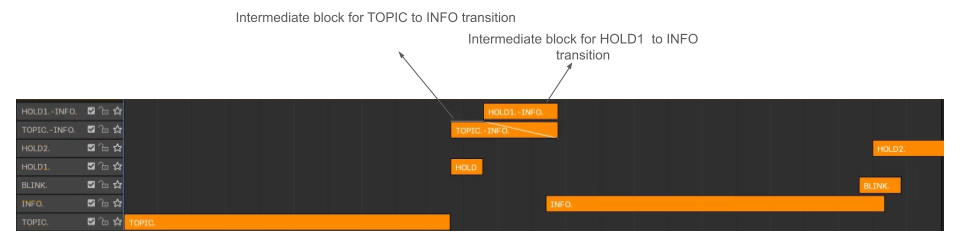
\includegraphics[width = 5in]{chapters/intermediate_blocks_pose_correction/images/info_about_intermediate_example.png}
    \caption{Intermediate Blocks for the AZee rule \emph{info-about(topic,info)}}
    \label{fig:info_about_intermediate_example}
\end{figure}

Simplest way to fill in intermediate blocks is to use linear or some other spline in these blocks. However, we propose the use of motion templates, which provide predefined motion patterns that can guide the interpolation within these blocks.

\subsection{Identifying Motion Templates}
\label{ch:intermediate_blocks_pose_correction:identifying_motion_templates}

Before filling in the intermediate blocks with some motion template, we need to identify them using an AZee template check (as discussed in section~\ref{ch:background_work:sign_language_descriptions:azee:templates} of chapter~\ref{ch:background_work}). The template check is a top-down search algorithm that selects the best motion template to match on the AZee expression. Figure~\ref{fig:top_down_search_template} shows the template check for the AZee expression \emph{info-about(cat,cute)}. The algorithm starts by searching for the most specific template that matches the expression, then gradually broadens the search until a suitable template is found.

\begin{figure}
    \centering 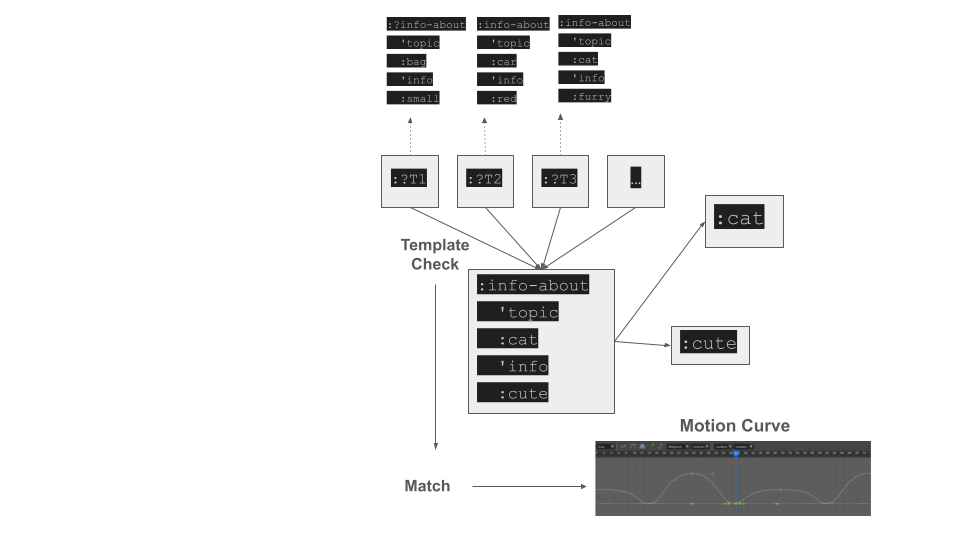
\includegraphics[width = 4in]{chapters/intermediate_blocks_pose_correction/images/top_down_search_template.png}
    \caption{Top-Down Search for Motion Template}
    \label{fig:top_down_search_template}
\end{figure}

\subsection{Creating Motion Templates}
\label{ch:intermediate_blocks_pose_correction:creating_motion_templates}

Motion templates (as discussed in section~\ref{ch:background_work:sign_language_synthesis:3d_techniques:avatar_animation:motion_templates} of chapter~\ref{ch:background_work}) are pre-defined motion patterns that guide the synthesis of new animations. In the context of AZee-driven synthesis, these templates serve as a blueprint for filling the intermediate blocks with relevant motion curves. For our experiments, we will be mainly using the \emph{40 brèves}~\cite{challant2022first} corpus. We chose to base this study on the first 5 rules in this corpus based on their frequency (see section  \ref{annex:intermediate_blocks_pose_correction:azee_rules_frequency} of annex).

Motion templates can be data-driven or artistic. Data driven templates are based on motion data extracted from the AZee rule and corresponding motion data. Artistically created templates, on the other hand, are designed by hand based on the AZee rule and desired motion features.

\paragraph{Data-Driven Motion Templates}
\label{ch:intermediate_blocks_pose_correction:creating_motion_templates:data_driven}

For creating data-driven templates, we first extract motion curves from the AZee annotated motion capture data. We use the Rosetta dataset~\cite{bertin2022rosetta} which is already AZee annotated. We choose to only include the upper body bones in the dataset since AZee doesn't contain lower body bones. Next, we retargeted the \gls{mocap} data on our BAZeel avatar, which is compatible with the AZee skeleton structure (figure~\ref{fig:retargeted}).

\begin{figure}
  \centering 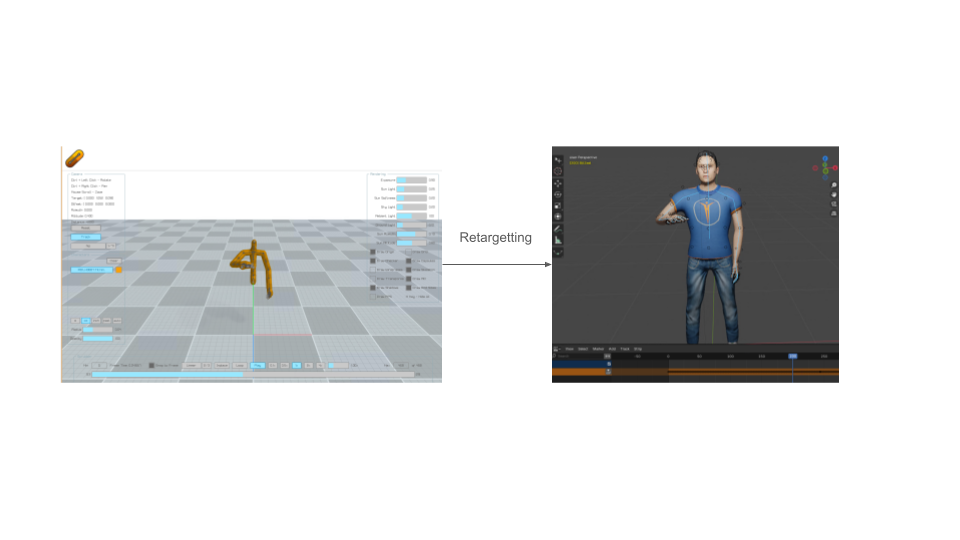
\includegraphics[width = 2.5in]{chapters/intermediate_blocks_pose_correction/images/retargeted.png}
  \caption{Retargeted mocap data to BAZeel avatar}
  \label{fig:retargeted}
\end{figure}

We converted the \gls{mocap} data into \gls{fk} pose arrays. The \gls{fk} pose array consists of the rotation values of each joint in the AZee skeleton (figure~\ref{fig:azee_fk_pose}). This representation is more suitable for our purposes since it allows us to directly create the templates based on the joint rotations.

\begin{figure}
  \centering 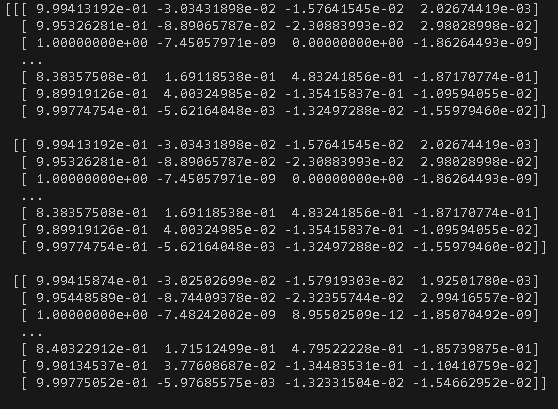
\includegraphics[width = 2.5in]{chapters/intermediate_blocks_pose_correction/images/azee_fk_pose.png}
  \caption{AZee FK Pose Array}
  \label{fig:azee_fk_pose}
\end{figure}

To create the templates we used the affected bone chains based on the low level description of the rule. For example, for the rule \emph{side-info}, we used the head, neck, and bust bones. We then extracted the motion curves for each bone and normalized them to the range \([-1, 1]\). The final blended rotations can be calculated using \gls{slerp} between the \( n \) quaternions \( q_1, q_2, \dots, q_n \):

\[
q_{\text{blend}} = \text{Slerp}\left(\dots \text{Slerp}\left(\text{Slerp}(q_1, q_2, t_1), q_3, t_2 \right) \dots , q_n, t_{n-1} \right)
\]

Where:
\begin{itemize}
    \item \( t_1, t_2, \dots, t_{n-1} \) are the blend factors for each interpolation step, with \( t_i \in [0, 1] \).
    \item The Slerp between two quaternions \( q_i \) and \( q_j \) is defined as:
    \[
    \text{Slerp}(q_i, q_j, t) = \frac{\sin((1-t)\theta)}{\sin(\theta)} q_i + \frac{\sin(t\theta)}{\sin(\theta)} q_j
    \]
    where \( \theta = \arccos(q_i \cdot q_j) \) is the angle between the quaternions.
\end{itemize}

Figure~\ref{fig:motion_curves_datadriven} shows template creation process.

\begin{figure}
    \centering 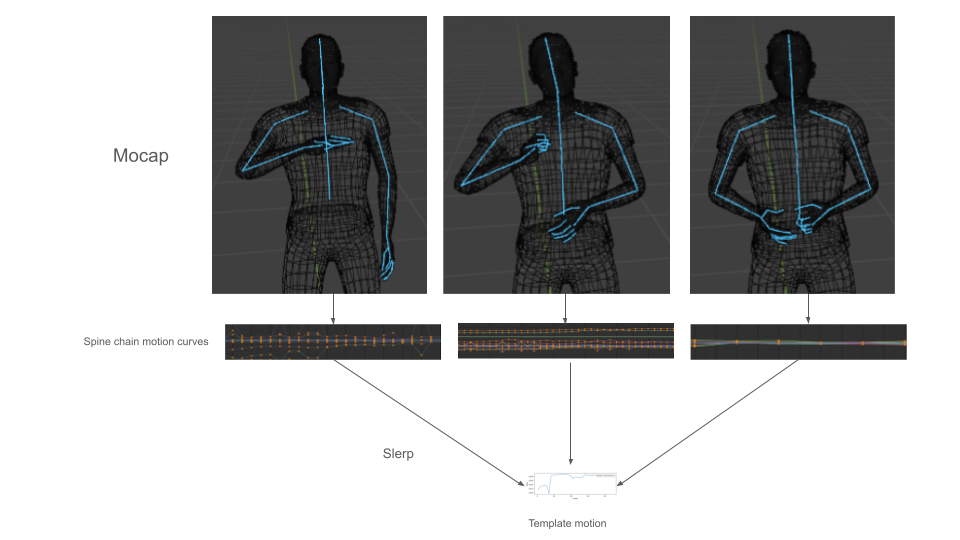
\includegraphics[width = 4in]{chapters/intermediate_blocks_pose_correction/images/motion_curves_template_datadriven.png}
    \caption{Data-Driven template creation for template \emph{side-info}}
    \label{fig:motion_curves_datadriven}
\end{figure}

\paragraph{Artistically Created Motion Templates}
\label{ch:intermediate_blocks_pose_correction:creating_motion_templates:artisitic}

Motion templates can also be created artistically, based on the linguistic context and the desired expressive qualities. Artistically created template for the rule \emph{about-ref} can be seen in figure~\ref{fig:motion_curves_template_artist}.

\begin{figure}
     \centering
    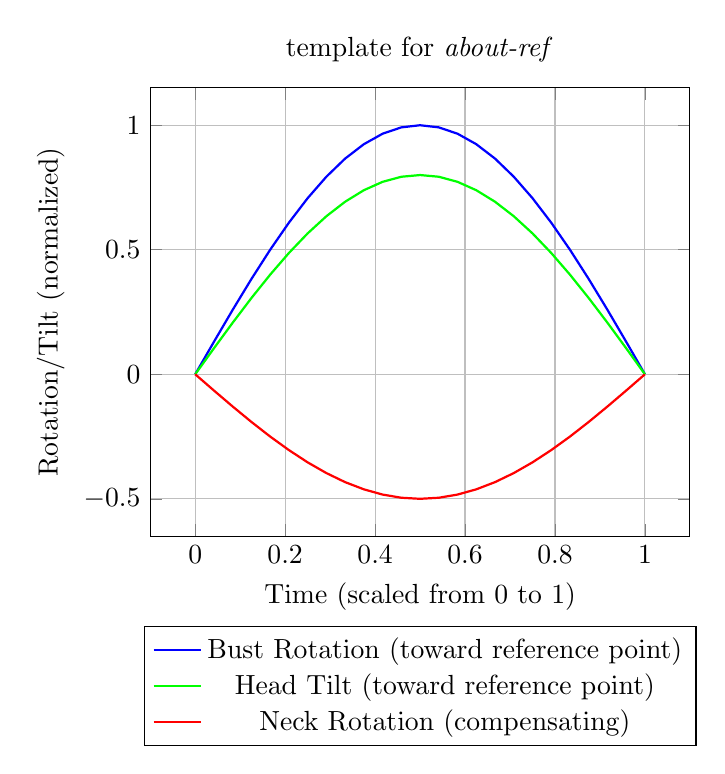
\begin{tikzpicture}
        \begin{axis}[
            title={template for \emph{about-ref}},
            xlabel={Time (scaled from 0 to 1)},
            ylabel={Rotation/Tilt (normalized)},
            grid=major,
            legend style={at={(0.5,-0.2)},anchor=north,legend columns=1} % Legend in two rows
        ]
        % Bust rotation
        \addplot[blue, thick, domain=0:1] {sin(deg(pi*x))};
        \addlegendentry{Bust Rotation (toward reference point)}
        
        % Head tilt
        \addplot[green, thick, domain=0:1] {0.8*sin(deg(pi*x))};
        \addlegendentry{Head Tilt (toward reference point)}
        
        % Neck rotation (compensating)
        \addplot[red, thick, domain=0:1] {-0.5*sin(deg(pi*x))};
        \addlegendentry{Neck Rotation (compensating)}
        
        \end{axis}
    \end{tikzpicture}
    \caption{Artistically Created motion curves for template \emph{about-ref}}
    \label{fig:motion_curves_template_artist}
\end{figure}

For reference, figure~\ref{fig:about_ref_irak} shows how the head and the spine chain move towards the reference point (\gls{rssp}), while the neck compensates for the rotation. The motion template reflects the same. 

\begin{figure}
    \centering 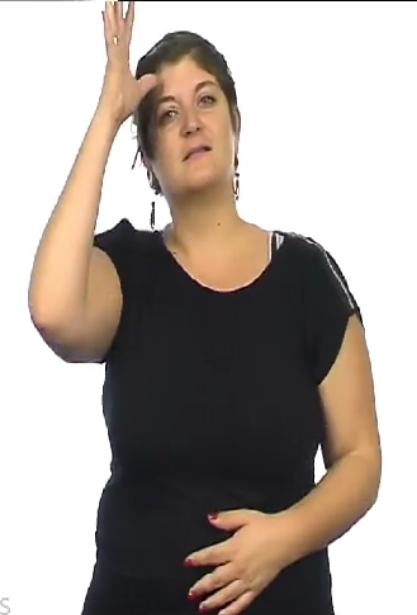
\includegraphics[width = 4in]{chapters/intermediate_blocks_pose_correction/images/about_ref_irak.png}
    \caption{Motion for the AZee rule \emph{about-ref(:irak, Rssp)}}
    \label{fig:about_ref_irak}
\end{figure}

\section{Pose Correction with AZee Low-Level synthesis}
\label{ch:intermediate_blocks_pose_correction:pose_correction_with_azee}

One part in enhancing the naturalness of \gls{sl} animations is to also ensure that the poses generated by the AZee system are contextually appropriate and realistic. Pose correction techniques can help achieve this by aligning the synthesized poses with the motion data in the dataset. In this section, we discuss the application of pose correction techniques to the AZee low-level synthesis system. By integrating pose correction, data-driven \gls{ik}, and latent space representations into the AZee framework, we aim to enhance the realism and expressiveness of \gls{sl} animations.

\subsection{Preparing the dataset}
\label{ch:intermediate_blocks_pose_correction:pose_correction_with_azee:dataset}

The first step in integrating pose correction into AZee is to train a \gls{vae} on a set of \gls{sl} poses. For this task, we use a dataset of \gls{mocap} data collected from the Rosetta dataset~\cite{bertin2022rosetta}. The dataset consists of 167066 poses which we assume to be representative enough to capture the diversity of poses and movements associated with different signs, providing a rich source of training data for the \gls{vae}. For training, we use the same \gls{fk} pose array representation as discussed in section~\ref{ch:intermediate_blocks_pose_correction:creating_motion_templates:data_driven}. We divided the dataset into training, validation, and test sets.

\subsection{Training VPoser}
\label{ch:intermediate_blocks_pose_correction:pose_correction_with_azee:training}

A \gls{vae} (earlier discussed in section~\ref{ch:background_work:sign_language_synthesis:3d_techniques:avatar_animation:deep_learning:latent_space} of chapter~\ref{ch:background_work}) is an autoencoder that learns a low-dimensional latent space representation of the input data. In the context of character animation, a \gls{vae} can be used to capture the distribution of poses in a dataset, allowing for the generation of new poses that are statistically similar to the training data. The \gls{vae} consists of an encoder network that maps input poses to a latent space and a decoder network that reconstructs the input poses from the latent space (figure~\ref{fig:vae}).

\begin{figure}[h]
\centering
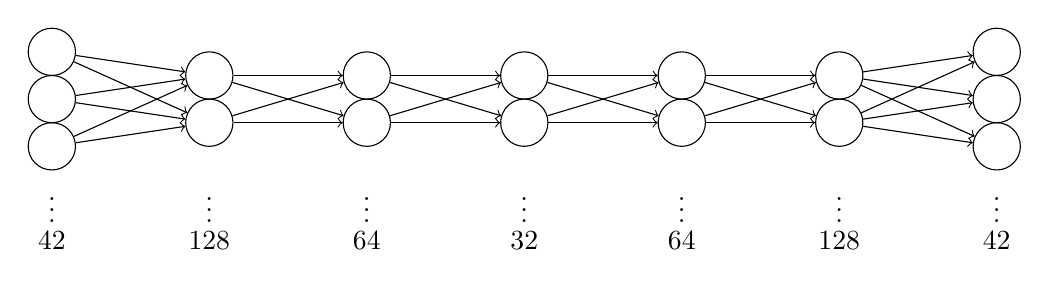
\begin{tikzpicture}[
    every neuron/.style={
        circle,
        draw,
        minimum size=0.6cm
    },
    neuron missing/.style={
        draw=none, 
        scale=1,
        text height=0.333cm,
        execute at begin node=\color{black}$\vdots$
    },
    layer/.style={
        rectangle,
        draw,
        text centered,
        minimum width=2cm
    }
]

% Input Layer
\foreach \i in {1,2,3}
    \node [every neuron/.try, neuron \i/.try] (input-\i) at (0,1.5-\i*0.6) {};

\node at (0,-1) {\vdots};
\node at (0,-1.5) {42};

% Encoder L1
\foreach \i in {1,2}
    \node [every neuron/.try, neuron \i/.try] (L1-\i) at (2,1.2-\i*0.6) {};

\node at (2,-1) {\vdots};
\node at (2,-1.5) {128};

% Encoder L2
\foreach \i in {1,2}
    \node [every neuron/.try, neuron \i/.try] (L2-\i) at (4,1.2-\i*0.6) {};

\node at (4,-1) {\vdots};
\node at (4,-1.5) {64};

% Latent Layer
\foreach \i in {1,2}
    \node [every neuron/.try, neuron \i/.try] (L3-\i) at (6,1.2-\i*0.6) {};

\node at (6,-1) {\vdots};
\node at (6,-1.5) {32};

% Decoder L4
\foreach \i in {1,2}
    \node [every neuron/.try, neuron \i/.try] (L4-\i) at (8,1.2-\i*0.6) {};

\node at (8,-1) {\vdots};
\node at (8,-1.5) {64};

% Decoder L5
\foreach \i in {1,2}
    \node [every neuron/.try, neuron \i/.try] (L5-\i) at (10,1.2-\i*0.6) {};

\node at (10,-1) {\vdots};
\node at (10,-1.5) {128};

% Output Layer
\foreach \i in {1,2,3}
    \node [every neuron/.try, neuron \i/.try] (output-\i) at (12,1.5-\i*0.6) {};

\node at (12,-1) {\vdots};
\node at (12,-1.5) {42};

% Draw the connections
\foreach \i in {1,2,3}
    \foreach \j in {1,2}
        \draw [->] (input-\i) -- (L1-\j);

\foreach \i in {1,2}
    \foreach \j in {1,2}
        \draw [->] (L1-\i) -- (L2-\j);

\foreach \i in {1,2}
    \foreach \j in {1,2}
        \draw [->] (L2-\i) -- (L3-\j);

\foreach \i in {1,2}
    \foreach \j in {1,2}
        \draw [->] (L3-\i) -- (L4-\j);

\foreach \i in {1,2}
    \foreach \j in {1,2}
        \draw [->] (L4-\i) -- (L5-\j);

\foreach \i in {1,2}
    \foreach \j in {1,2,3}
        \draw [->] (L5-\i) -- (output-\j);

\end{tikzpicture}
\caption{Architecture of the VAE}
\label{fig:vae}
\end{figure}

During training, batches of poses are processed, with each batch consisting of 512 samples. The training is carried out on a CUDA-enabled GPU, utilizing mixed precision training for efficiency. The \gls{vae} architecture consists of a latent space with 32 dimensions, and the neural network has 512 neurons per layer. 

The loss function used during training includes two primary components: 
\begin{itemize}
    \item \textbf{Reconstruction Loss}: This loss is computed at the joint level by comparing the reconstructed pose with the original pose using L1 loss. An additional pose-level reconstruction loss (L2 loss) is applied during the first 10 epochs to help the model learn better early on.
    \item \textbf{KL Divergence Loss}: The KL divergence regularizes the latent space by enforcing it to follow a standard normal distribution, ensuring that the latent space representation is smooth and continuous.
\end{itemize}

The total loss is the sum of the reconstruction loss and KL divergence loss. The optimization is carried out using the Adam optimizer with a learning rate of $1 \times 10^{-2}$ and weight decay of $0.0001$. A learning rate scheduler is used, which reduces the learning rate by a factor of 0.5 every third of the training epochs. 

\subsection{Implementing Pose Correction}
\label{ch:intermediate_blocks_pose_correction:pose_correction_with_azee:implementation}

With the \gls{vae} trained, we can now implement a pose correction system that leverages the learned latent space to match poses generated by the AZee system to the most appropriate pose in the dataset.

Algorithm~\ref{alg:pose_correction} outlines the pose correction process. Given a target pose generated by the AZee synthesizer, we first encode the pose into the latent space using the VPoser encoder. We then compute the distance between the encoded pose and each pose in the dataset, selecting the pose with the smallest distance as the best match. Finally, we decode the matched pose back into the AZee \gls{fk} pose array and apply it to the character.

\begin{algorithm}
  \caption{AZee constraint optimization with pose correction algorithm}
  \label{alg:pose_correction}
  \begin{algorithmic}[1]
  \For{$frame$ \textbf{in} frames}
      \State \texttt{switch\_cursor\_to\_frame($f$)}
      \For{\texttt{parallel\_block \textbf{in} self.parallel\_blocks}}
          \State \texttt{constraints.add(parallel\_block.constraints)}
      \EndFor
      \For{\texttt{constraint \textbf{in} constraints}}
          \State \texttt{constraint.apply($frame$)}
      \EndFor
      \State \texttt{model.pose\_embedding}
      \State \texttt{model.global\_trans}
      \State \texttt{optimizer = \dots}
      \For{\texttt{epoch \textbf{in} range(max\_epochs)}}
          \State \texttt{optimizer.zero\_grad()}
          \State \texttt{\dots}
          \State \texttt{optimizer.step()}
          \If{\texttt{loss.item() < threshold}} \State \texttt{break} \EndIf
      \EndFor
      \State \texttt{posture.keyframe($frame$)}
  \EndFor
  \end{algorithmic}
  \end{algorithm}

\section{Results and Implementation}
\label{ch:intermediate_blocks_pose_correction:results}

\subsection{Results and Implementation for Intermediate Block Generation}
\label{ch:intermediate_blocks_pose_correction:results:intermediate_block_generation}

We chose to extend our previous animator in blender to include the intermediate block generation process. The intermediate blocks are represented as strips in the \gls{nle}.

Table~\ref{tab:intermediate_blocks} shows the results of the intermediate block generation process. The table shows the motion curve profiles for the most common AZee rules.

\begin{longtable}{|c|c|}
    \caption{Motion curves of some intermediate blocks for some AZee rules}
    \label{tab:intermediate_blocks}
    \hline
    \textbf{AZee Rule} & \textbf{Template} \\
    \hline
    \endfirsthead
    \emph{info-about} & 
    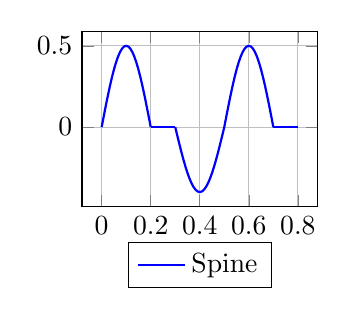
\begin{tikzpicture}
        \begin{axis}[
            grid=major,
            width=1.8in,
            height=1.5in,
            axis line style={-stealth},
            xtick={},
            ytick={},
            legend style={at={(0.5,-0.2)},anchor=north,legend columns=1}
        ]
        \node[anchor=west] at (rel axis cs:1,0) {t}; % Label 't' at the end of x-axis
        % Signing phase
        \addplot[blue, thick, domain=0:0.2] {0.5*sin(deg(5*pi*x))};
        
        % Hold phase 1
        \addplot[blue, thick, domain=0.2:0.3] {0};
        
        % Relaxation phase
        \addplot[blue, thick, domain=0.3:0.5] {-0.4*sin(deg(5*pi*(x-0.3)))};
        
        % Signing phase 2
        \addplot[blue, thick, domain=0.5:0.7] {0.5*sin(deg(5*pi*(x-0.5)))};
        
        % Hold phase 2
        \addplot[blue, thick, domain=0.7:0.8] {0};
        \addlegendentry{Spine}
        \end{axis}
    \end{tikzpicture} \\
    \hline
    \emph{side-info} & 
    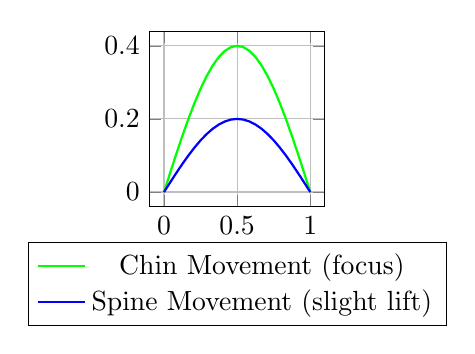
\begin{tikzpicture}
        \begin{axis}[
            grid=major,
            width=1.5in,
            height=1.5in,
            axis line style={-stealth},
            xtick={},
            ytick={},
            legend style={at={(0.5,-0.2)},anchor=north,legend columns=1}
        ]
        \node[anchor=west] at (rel axis cs:1,0) {t}; % Label 't' at the end of x-axis
        % Chin and spine movement
        \addplot[green, thick, domain=0:1] {0.4*sin(deg(pi*x))}; 
        \addlegendentry{Chin Movement (focus)}
        
        \addplot[blue, thick, domain=0:1] {0.2*sin(deg(pi*x))};
        \addlegendentry{Spine Movement (slight lift)}
        \end{axis}
    \end{tikzpicture} \\
    \hline
    \emph{about-ref} & 
    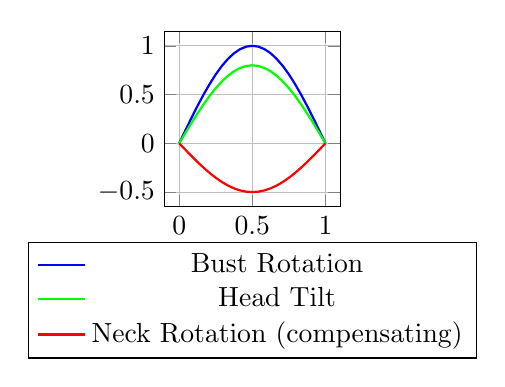
\begin{tikzpicture}
        \begin{axis}[
            grid=major,
            width=1.5in,
            height=1.5in,
            axis line style={-stealth},
            xtick={},
            ytick={},
            legend style={at={(0.5,-0.2)},anchor=north,legend columns=1}
        ]
        \node[anchor=west] at (rel axis cs:1,0) {t}; % Label 't' at the end of x-axis
        % Bust, head tilt, and neck rotation
        \addplot[blue, thick, domain=0:1] {sin(deg(pi*x))};
        \addlegendentry{Bust Rotation}
        
        \addplot[green, thick, domain=0:1] {0.8*sin(deg(pi*x))};
        \addlegendentry{Head Tilt}
        
        \addplot[red, thick, domain=0:1] {-0.5*sin(deg(pi*x))};
        \addlegendentry{Neck Rotation (compensating)}
        \end{axis}
    \end{tikzpicture} \\
    \hline
    \emph{instance-of} & 
    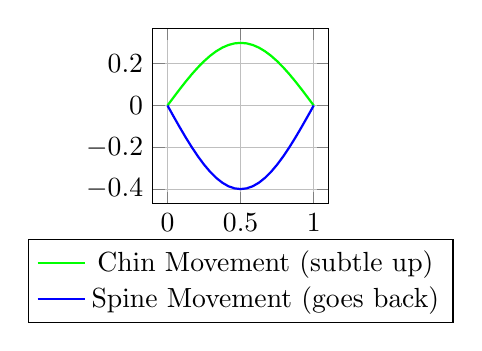
\begin{tikzpicture}
        \begin{axis}[
            grid=major,
            width=1.5in,
            height=1.5in,
            axis line style={-stealth},
            xtick={},
            ytick={},
            legend style={at={(0.5,-0.2)},anchor=north,legend columns=1}
        ]
        \node[anchor=west] at (rel axis cs:1,0) {t}; % Label 't' at the end of x-axis
        % Chin movement (subtle) and spine movement (back)
        \addplot[green, thick, domain=0:1] {0.3*sin(deg(pi*x))}; 
        \addlegendentry{Chin Movement (subtle up)}
        
        \addplot[blue, thick, domain=0:1] {-0.4*sin(deg(pi*x))};
        \addlegendentry{Spine Movement (goes back)}
        \end{axis}
    \end{tikzpicture} \\
    \hline
    \emph{in-context} & 
    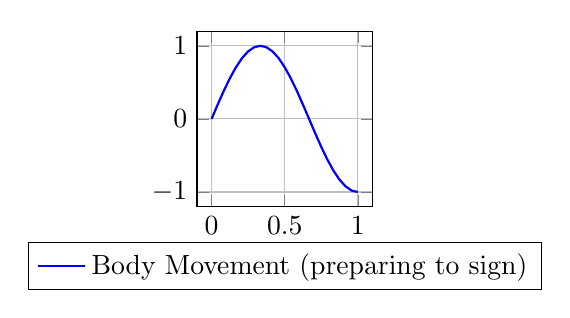
\begin{tikzpicture}
        \begin{axis}[
            grid=major,
            width=1.5in,
            height=1.5in,
            axis line style={-stealth},
            xtick={},
            ytick={},
            legend style={at={(0.5,-0.2)},anchor=north,legend columns=1}
        ]
        \node[anchor=west] at (rel axis cs:1,0) {t}; % Label 't' at the end of x-axis
        % Body preparation for signing
        \addplot[blue, thick, domain=0:1] {sin(deg(1.5*pi*x))};
        \addlegendentry{Body Movement (preparing to sign)}
        
        \end{axis}
    \end{tikzpicture} \\
    \hline
\end{longtable}

We compare the results of using standard interpolation techniques with the proposed template-based interpolation method in the video~\footnote{\url{https://www.phd.paritosh-sharma.com/dissertation/ch5_templates.mp4}}.

An increase in naturalness when animating using the intermediate blocks technique can be seen. Moreover, this work provides us inights regarding the motion profile which an AZee rule abstracts.

\subsection{Results and Implementation for Pose Correction}
\label{ch:intermediate_blocks_pose_correction:results:intermediate_block_generation}

We created the pose corrector as a separate module in the existing AZee animator. The pose corrector is responsible for matching the poses generated by the AZee system to the most appropriate pose in the dataset. As the algorithm~\ref{alg:pose_correction} shows, the pose correction process is applied just after the AZee constraints are optimized.

Snapshots with standard synthesis and synthesis with pose correction and the corresponding AZee code for the same are shown in table~\ref{tab:results}.

\begin{table}
  \centering
  \begin{tabular}{|c|c|c|}
    \hline
    \textbf{Standard Synthesis} & \textbf{Synthesis with Pose Correction} & \textbf{AZee Code} \\
    \hline
    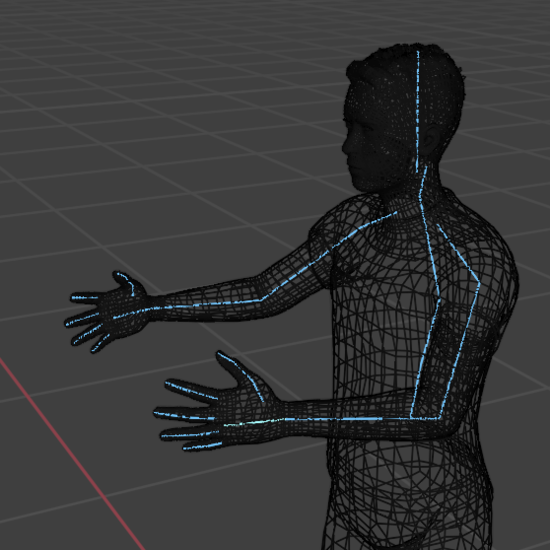
\includegraphics[width = 1.5in]{chapters/intermediate_blocks_pose_correction/images/standard_synthesis_armoire.png} & 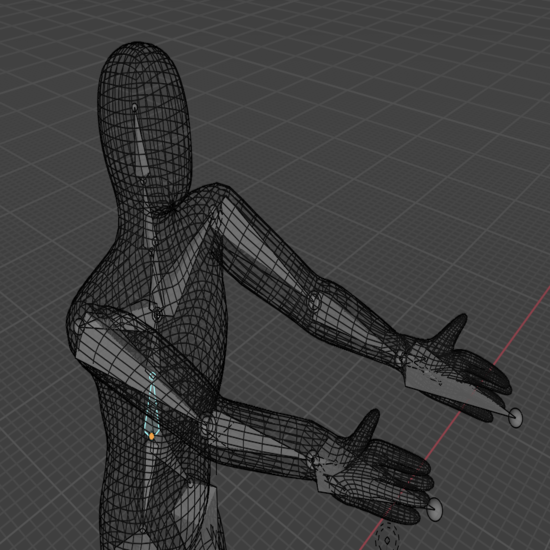
\includegraphics[width = 1.5in]{chapters/intermediate_blocks_pose_correction/images/pose_correction_synthesis_armoire.png} & 
      \emph{:armoire} \\
    \hline
    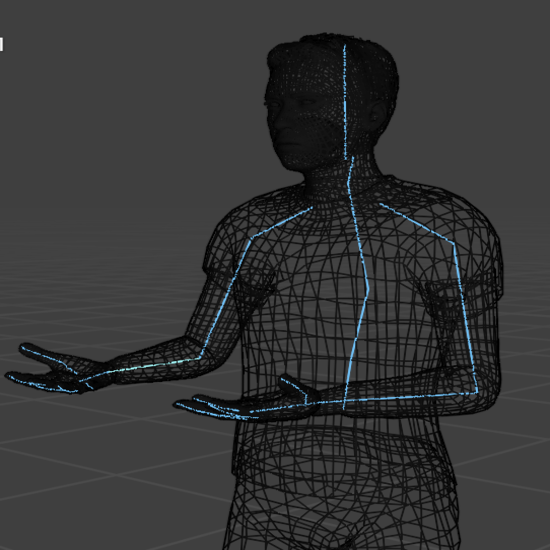
\includegraphics[width = 1.5in]{chapters/intermediate_blocks_pose_correction/images/standard_synthesis_maintenant.png} & 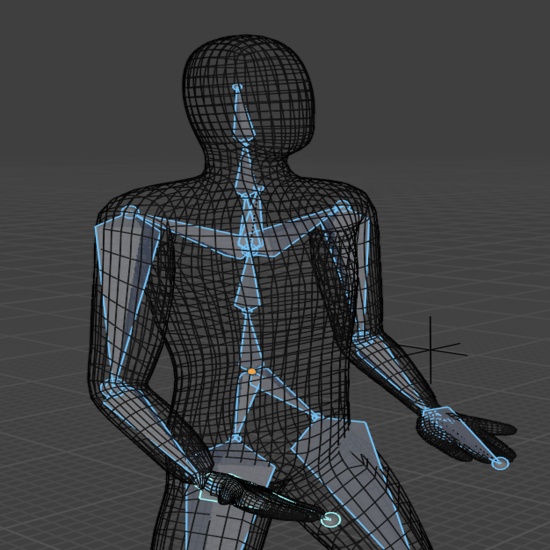
\includegraphics[width = 1.5in]{chapters/intermediate_blocks_pose_correction/images/pose_correction_synthesis_maintenant.png} &
      \emph{:maintenant} \\
    \hline
    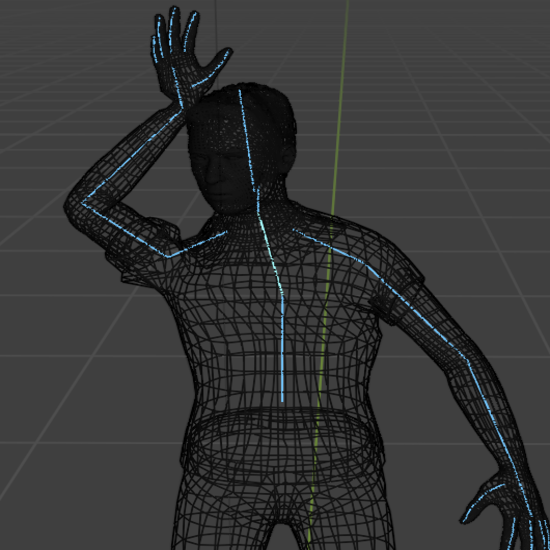
\includegraphics[width = 1.5in]{chapters/intermediate_blocks_pose_correction/images/standard_synthesis_abt_ref_irak.png} & 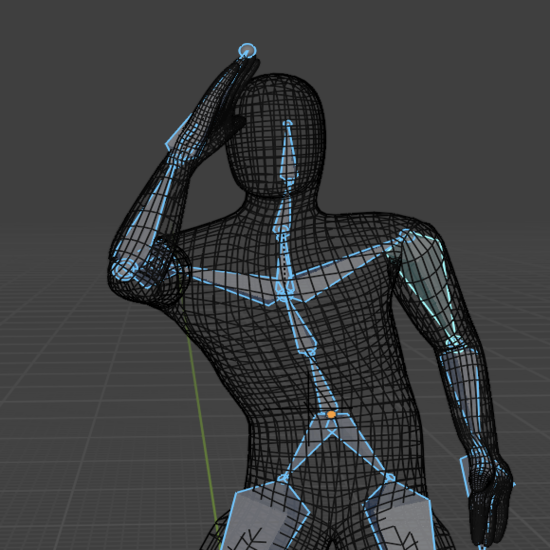
\includegraphics[width = 1.5in]{chapters/intermediate_blocks_pose_correction/images/pose_correction_synthesis_abt_ref_irak.png} &
      \emph{:about-ref(:irak, Rssp)} \\
    \hline
  \end{tabular}
  \caption{Comparison of standard synthesis and synthesis with pose correction}
  \label{tab:results}
\end{table}

The pose correction system seems to produces more natural and contextually appropriate animations compared to standard joint-limit based synthesis. However, due to retargeting losses, the integration of pose correction into \gls{sl} synthesis is still in the early stages. We also observe that the corrector might change the pose of the character in a way that is not always desirable~\ref{fig:problem_pose_correction}.

\begin{figure}
  \centering 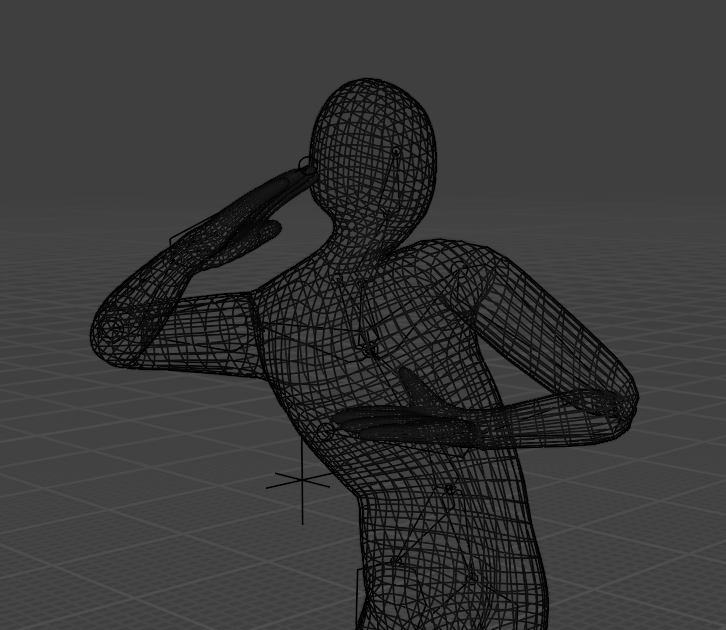
\includegraphics[width = 2.5in]{chapters/intermediate_blocks_pose_correction/images/problem_pose_correction.png}
  \caption{Problems with current correction module}
  \label{fig:problem_pose_correction}
\end{figure}

Lastly, figure~\ref{fig:losses} shows how retargeting the \gls{mocap} data to the AZee skeleton structure results in a loss of information. This loss can affect the quality of the generated animations and is an area for future improvement.

\begin{figure}
  \centering 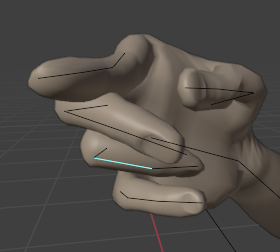
\includegraphics[width = 2.5in]{chapters/intermediate_blocks_pose_correction/images/losses.png}
  \caption{Retargeting losses for pointing on the Rssp}
  \label{fig:losses}
\end{figure}

\section{Conclusion and Future Work}
\label{ch:intermediate_blocks_pose_correction:conclusion_and_future_work}

In this chapter, we explored techniques to make our synthesis system more natural. By leveraging the AZee model and existing motion data, we were able to fill in the gaps left by the linguistic model and create more expressive and coherent animations. 

%limitations
While the current system of motion templates proves effective for generating smooth transitions in most body movements, it faces significant challenges when dealing with finer details such as finger articulation. The complexity of finger movements in \gls{sl}, especially during rapid transitions, requires high precision in motion curves and templates. Unfortunately, the current implementation lacks the necessary granularity, resulting in robotic transitions. Moreover, capturing thte nuances of coarticulation between handshapes be it with \gls{mocap} or using artistic templates an open challenge. Another limitation stems from too much data in the motion templates. This might bring in information such as the identity of the signer, which may not always generalize well. This can be mitigated by using a more generalized set of motion templates that can be applied across different signing scenarios.

Similarly, while the integration of pose correction into \gls{sl} synthesis in out animator, it also introduces new challenges. Data-driven and latent space methods typically require significant computational resources, both during training and inference. This can be a major barrier in applications where low latency is critical. Also the effectiveness of deep learning models depends heavily on the availability of high-quality training data. In many cases, obtaining sufficient \gls{mocap} data can be difficult, especially for non-standard or stylized animations. Lastly, while deep learning models can generate realistic and high-quality animations, they often lack the fine-grained control that human animators require. Ensuring that these models produce outputs that align with artistic vision remains a significant challenge.

Future areas to improve our work technique could include a more detailed quantitative analysis of motion capture data based on a broader range of AZee rules, as well as further refinement of finger tracking and facial expressions in the motion templates. Since obtaining good quality \gls{mocap} data is also a challenge, pose estimation based on image data could be explored as an alternative~\ref{annex:intermediate_blocks_pose_correction:pose_est_templates}. Since, motion curves for intermediate blocks might not have one-to-one correspondence with the AZee rules, newer techniques such as Diffusion based inbetweening~\cite{cohan2024flexible} could also be used for better intermediate block generation. 

Similarly, newer posers based on neural distance fields~\cite{tiwari2022pose} or diffusion~\cite{lu2023dposer} could be used for pose correction since the current poser has a bayesian bias. Also, continuity of the trained model with respect to signing spaces could be studied further improving the the learnt pose prior. Lastly, since natural human gestures are independant of the language, a more generalized pose correction model could be trained on a more generalized dataset.

\end{document}